\documentclass{article}
\usepackage[utf8]{inputenc}
\usepackage{amsmath, amsfonts,fullpage}
\usepackage{graphicx}
\title{Latex Homework 9th Grade\\  Week 1 - Intro to LaTeX}
\author{Aditya Velusamy, Kayla Dayman, Ian To}
\date{Edited \today}
\newcommand{\quadform}{$x=\frac{-b\pm\sqrt{b^2-4ac}}{2a}$}
\begin{document}

\maketitle

\section{Bio: Aditya Velusamy}
I am Aditya Velusamy. I am in 9th grade and a linux enjoyer(currently a Linux Mint user but I have used Manjaro and Debian). I enjoy tinkering with computers and technology. I hope that in this class I can get more proficient with LaTeX as well as explore more areas of maths.
\section{Bio: Kayla Dayman}
I am Kayla Dayman, I'm currently a freshman and I am not an interesting person. My main hobby is crochet, which I've been doing for about five and a half years. I also got a 5 on the AP Calculus BC test. I hope to become a bigger nerd than I already am over the course of the year.
\section{Bio: Ian To}
I am Ian To, a freshman currently in class standing. I enjoy doing music and code, with music I've been doing since I was around 2 years old. I hope that in this class I can become
good at using LaTeX and know more math topics.
\section{Quadratic Formula Macro}
\quadform
\section{Group Picture}
\begin{figure}
\centering
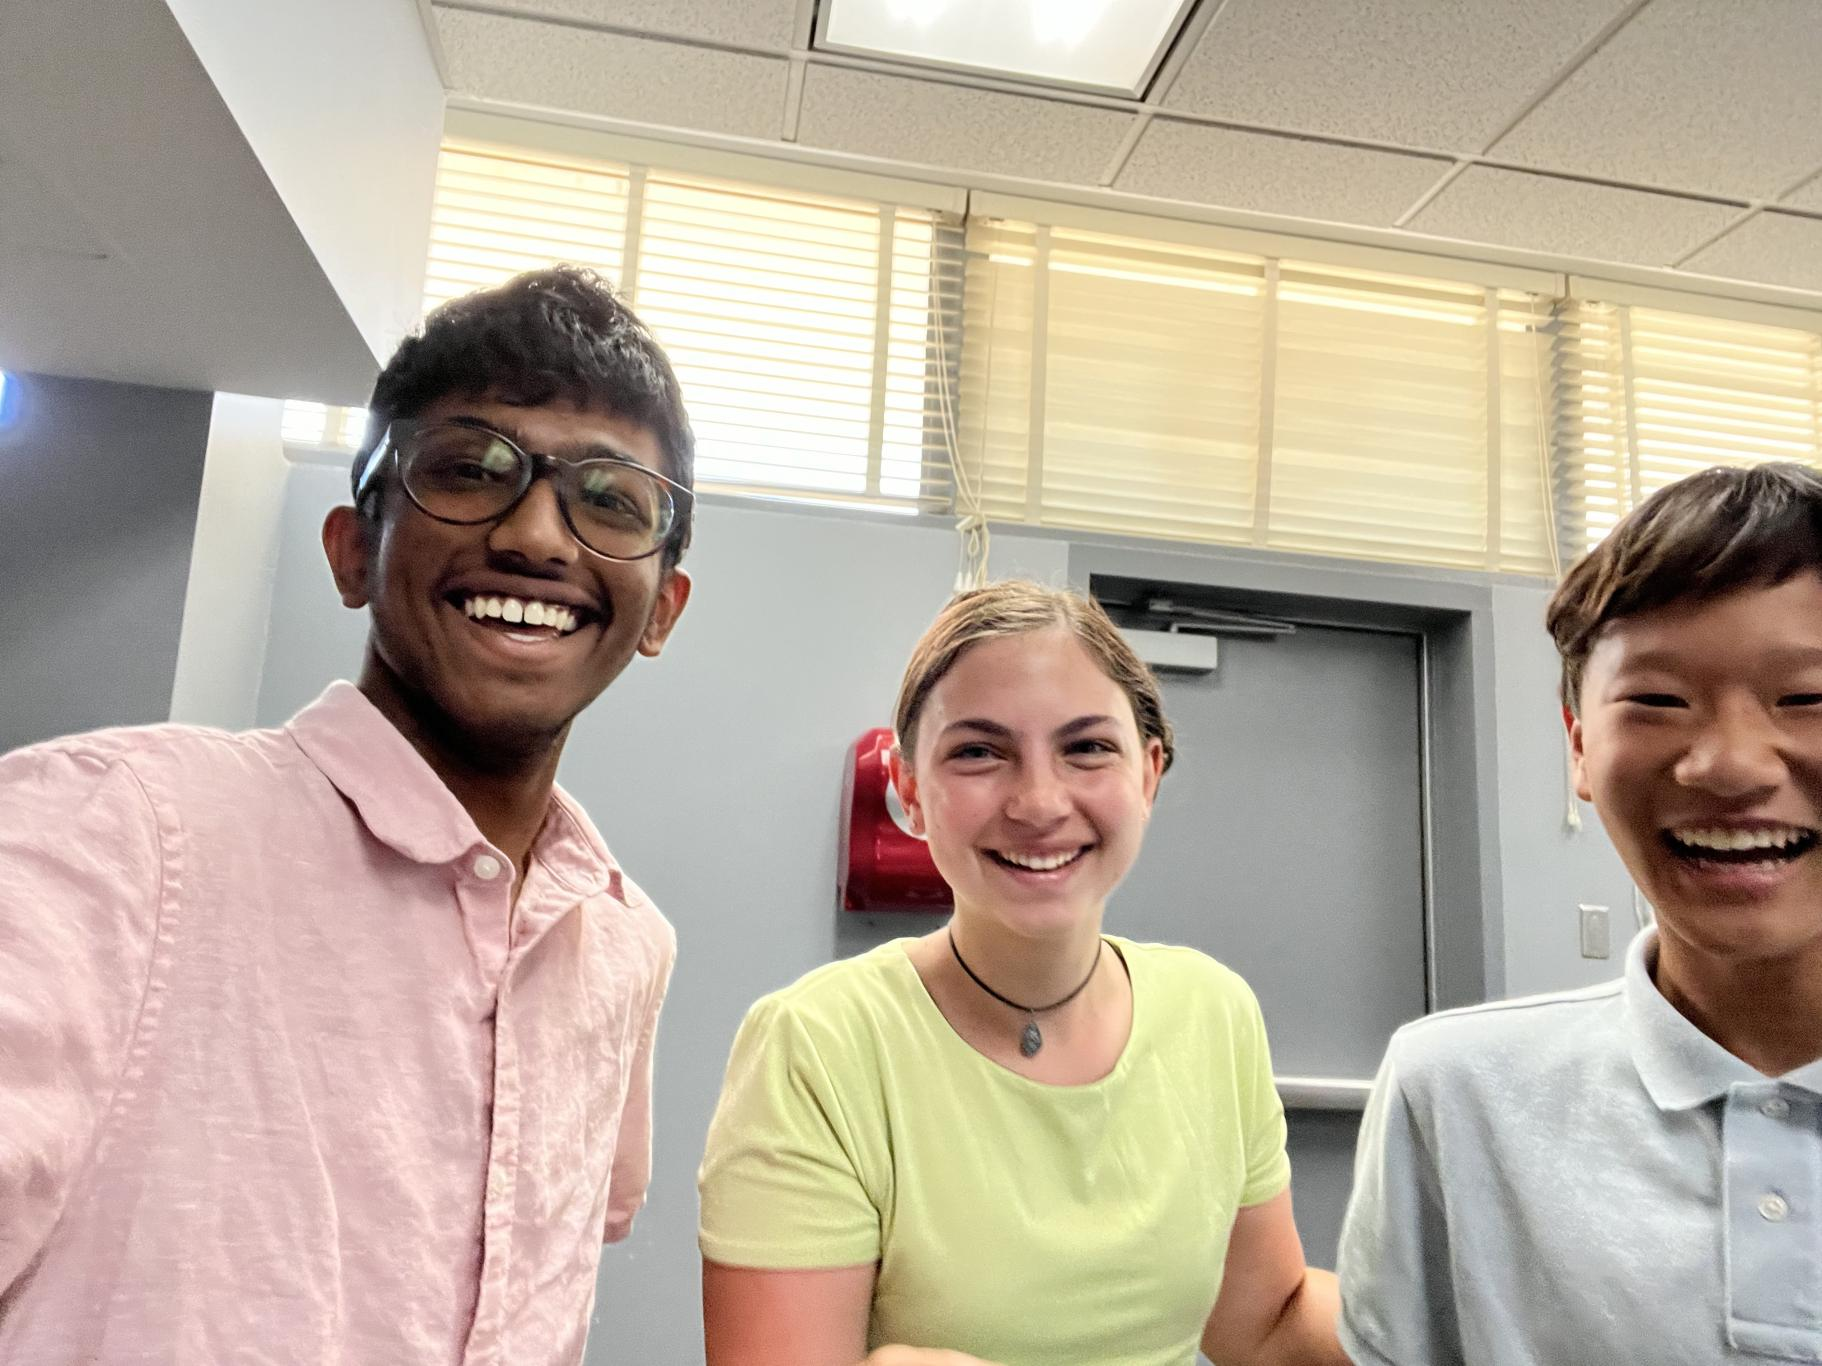
\includegraphics[scale=0.2]{./IMG_1617.jpg}
\end{figure}
\end{document}
